% !TeX spellcheck = en_GB
\setcounter{section}{-1}
\section{Introduction}

Fractals have fascinated mathematicians for over a century.
However, in this paper, we intend to study the properties of fractals in order to use this theory for physics model of porous materials.

We will first recall some background theory on set dimensionality and fractals.
We use this theory as a tool to study basic properties of percolation fractals.
Percolation fractals are obtained from applying a process called "filtration" on an initial set.
During this process, we randomly remove some parts of the initial set.
Percolation fractals are of two main types: classical ones, where only one filtration is performed, and recursive ones, where filtrations are performed recursively on the remaining subset.

Our goal will be to have a better understanding of the structure arising from these processes.
Keeping in mind the physical interpretation, we will be particularly interested in how particles may travel inside this medium.

First, we will turn our interest to the size of the central connected structure (the "blob") of the percolation.
Later, we will be more particularly interested in the existence of crossings path of the medium.
Indeed, a crossing path in a physical material enables a fluid to traverse the porous medium.

Some papers were already published, and some theory is already known.
However, the vast majority of the literature concentrates on the case of a percolation initialized by a square in two dimensions.
Given the three dimensionality of our world, it is interesting to extend the study (at least) to this third dimension.
We will extend some results known in two dimensions to any dimension.

Finally, despite the elegance of the theoretical results, they only treat extreme cases (i.e. probability parameter very low or very high).
To get an understanding of the behaviour for more moderate parametrisations, we will use numerical experiments.
In order to have the best accuracy possible, we developed a neat and efficient algorithm.
To avoid mixing mathematics with too deep numerical considerations, the algorithmic explanation part has been moved to the appendix (see \ref{algorithms}).

\begin{figure}[!h]
	\vspace{2cm}
	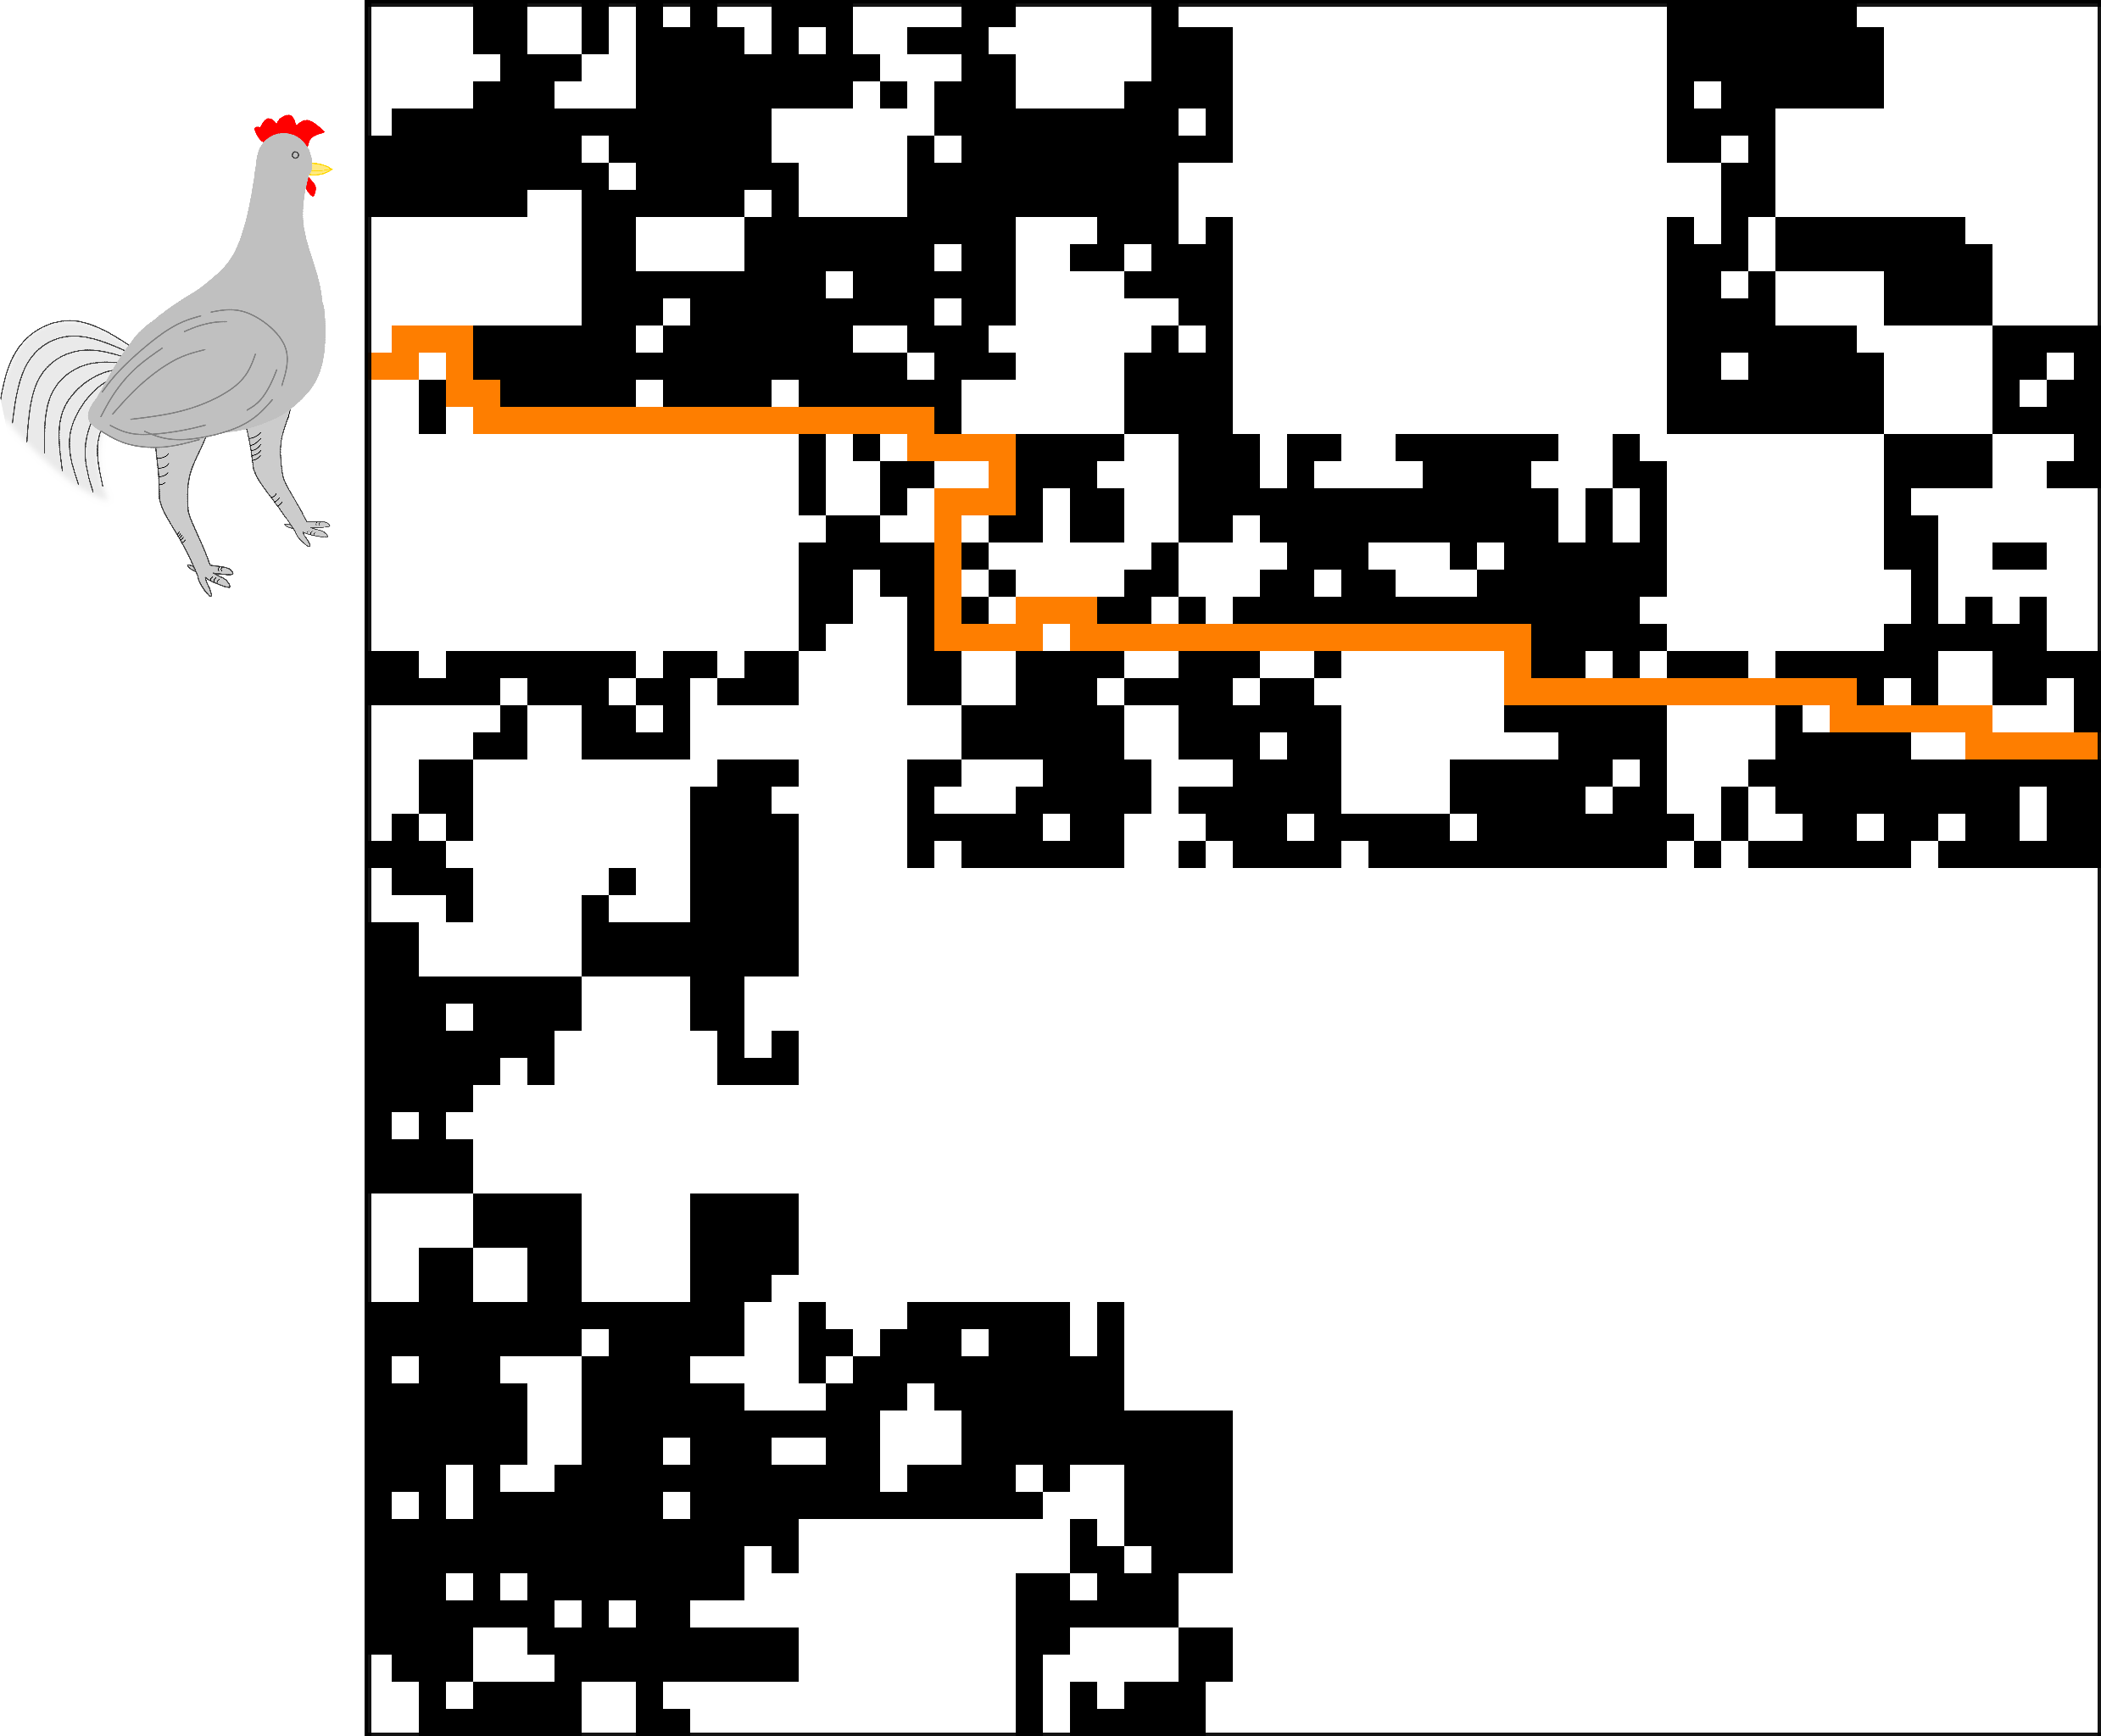
\includegraphics[height=8cm]{intro_picture}
	\centering
	\caption{Illustration of a chicken crossing a percolation (in reference to the title)}
	\label{fig:introRecursivePercolation}
\end{figure}
